\begin{center}
        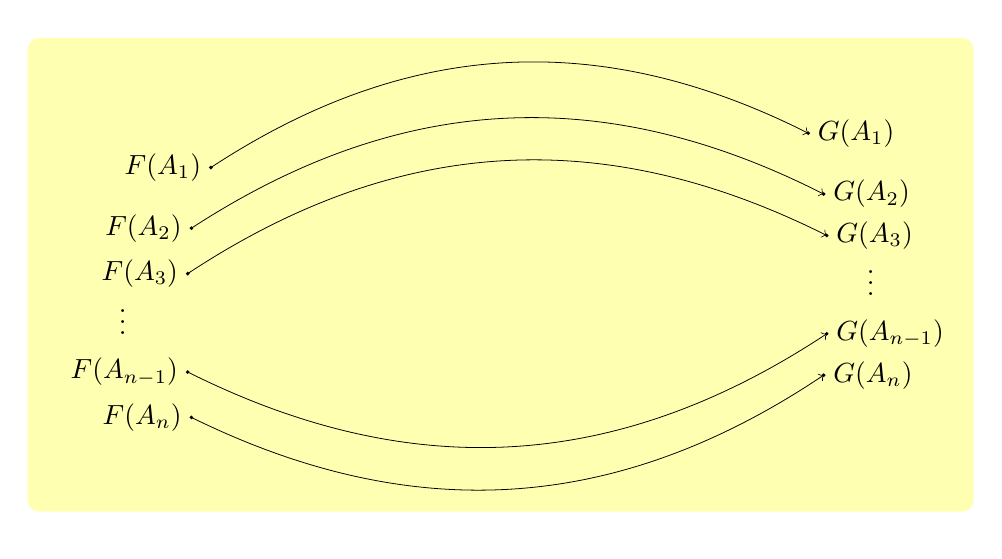
\begin{tikzpicture}
            \filldraw[rounded corners, Yellow!30]
            (-5,-4) rectangle (7, 2);
    
            \begin{scope}[xshift = 0.2cm, yshift=1cm]
                \coordinate (A) at (-2, 0.03);
                \coordinate (a) at (-2, -4);
        
                \coordinate (B) at (4, 1);
                \coordinate (b) at (4, -4);
                
                \foreach \t/\tt in {5/1, 8/2, 10/3}{
                    \pgfmathsetmacro{\n}{\t*0.05}
                    
                    \path (A) to[bend right = 85] coordinate[pos = \n] (A\t) (a);
                    \path (B) to[bend left = 40] coordinate[pos = \n] (B\t) (b);
                    
                    \filldraw (A\t) circle (0.1ex) node[left]{$F(A_{\tt})$};
                    \filldraw (B\t) circle (0.1ex) node[right]{$G(A_{\tt})$};
                    
                    \draw[line width = 0.1mm, ->] (A\t) to[bend left] (B\t);
                }
                \node at (-4,-2.5) {$\vdots$}; 
                \node at (5.5,-2) {$\vdots$}; 
                \begin{scope}[yshift=-1.25cm]
                    \coordinate (A) at (-2, 0.03);
                    \coordinate (a) at (-2, -4);
        
                    \coordinate (B) at (4, 1);
                    \coordinate (b) at (4, -4);
                    \foreach \t/\tt in {10/{n-1}, 12/{n}}{
                    \pgfmathsetmacro{\n}{\t*0.05}
                    
                    \path (A) to[bend right = 85] coordinate[pos = \n] (A\t) (a);
                    \path (B) to[bend left = 40] coordinate[pos = \n] (B\t) (b);
                    
                    \filldraw (A\t) circle (0.1ex) node[left]{$F(A_{\tt})$};
                    \filldraw (B\t) circle (0.1ex) node[right]{$G(A_{\tt})$};
                    
                    \draw[line width = 0.1mm, ->] (A\t) to[bend right] (B\t);
                }
                \end{scope}
            \end{scope}
        \end{tikzpicture}
    \end{center}